\subsection{Machine learning}
Le machine learning ou en bon français apprentissage automatique est l'élaboration d'algorithmes capable d'apprendre en étudiant des exemples. Il est la branche principale de l'intelligence artificielle. Le machine learning est particulièrement bien adapté à la reconnaissance d'image et ainsi à la détection de pièces de monnaie. 
\subsubsection{Principe général}
Le machine learning est constitué de deux étapes principales.
\begin{enumerate}
\item Phase d'apprentissage : l'algorithme traite des milliers d'information d'une base de donnée. Il reçoit une entrée $X$ dont il connaît la sortie $Y$. Lors de cette phase, l'algorithme va analyser les corrélations qui lient les entrées $X$ aux sorties $Y$. Il va en déduire de lui-même les caractériques importantes de cette liaison.
\item Phase de prédiction : l'algorithme reçoit une nouvelle entrée $X$, il la compare à celles qui l'a analysées et ainsi, il doit prédire la sortie $Y$. 
\end{enumerate}
Dans notre cas, l'entrée $X$ est l'image d'une pièce de monnaie et la sortie $Y$ la valeur de la pièce. L'algorithme va s'entrainer à reconnaître une pièce de monnaie et à les distinguer les unes des autres en analysant des milliers d'images d'une base de donnée. Ainsi, il sera capable face à une nouvelle image d'en déduire la valeur de la pièce. 
\subsubsection{Application détaillée du principe}
Le machine learning peut être détaillé en 7 étapes et ainsi être mieux expliqué.
\begin{enumerate}
\item  Rassemblement de données : actuellement, il existe des milliers de base de donnée regroupant chacune d'elle des milliers d'images. Cette première étape consiste à rassembler les images qui nous intéressent.
\item  Préparation des données : c'est l'encodage et la détermination de l'entrée X et de la sortie Y. On doit imaginer pouvoir interpréter les données par un repère et des axes X et Y.
\item Choix du modèle : le modèle est un algorithme mathématique avec un certain nombre de paramètres qui doivent être appris à partir de données. La partie essentielle du machine Learning est de trouver un modèle qui puisse correspondre au mieux à ces données. 
\item  Entrainement :  le but de l’entrainement est de crée un model précis qui puisse répondre à notre question de façon fiable. 
On a besoin de données pour entrainer le module. On va prendre des caractéristiques de l’object que l'on veut reconnaitre (taille, forme couleur,…).
\begin{center}
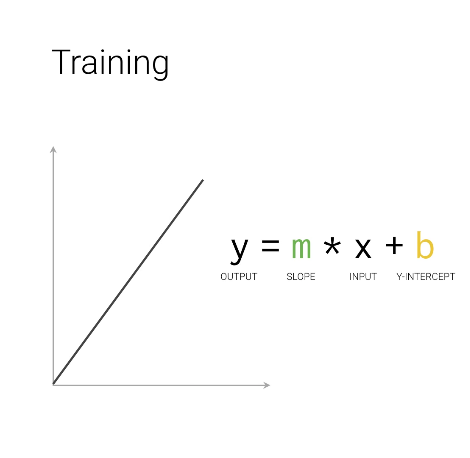
\includegraphics[height=5.5cm]{images/ml1_1.png}
\end{center}

On place les paramètres sur droite $d \equiv y = mx+b$ où
$$\begin{cases}x$ est l’entrée$ \\
m$ est la pente$ \\
b$ est l'ordonnée à l'origine$ \\
y$ est la valeur de $d$ en un point précis, c'est la sortie$
\end{cases}$$


Pour modifier la position de la droite, on joue sur les paramètres $m$ et $b$ ($m$ et $b$ sont les différentes valeurs des caractéristiques). Pour que le système puisse assimiler toute l’information, on utilise des matrices. 
La matrice des $m$ est la matrice des poids (\textit{weights}) et la matrice des $b$ est la matrice des biais (\textit{biases}). 

\begin{center}
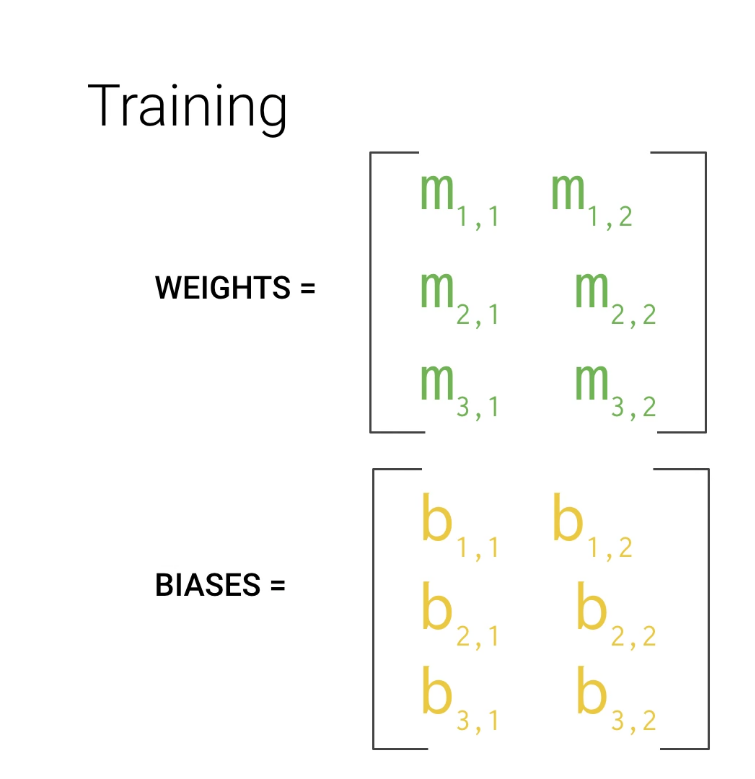
\includegraphics[height=7.5cm]{images/ml1_2.png}
\end{center}

Il faut un système avec tous les paramètres $m$ et tous les paramètres $b$ et le but est de, en faisant varier les paramètres, entrainer le système à reconnaitre et à faire des prédictions de plus en plus fiable.

\item Evalutation : après l’entrainement, une évaluation du système avec des nouvelles données nous aide à voir le pourcentage de fiabilité du module.

\item Paramètre et hyperparamètre : ce sont deux types de paramètre. Ces paramètres expriment les propriétés de «niveau supérieur» du modèle telles que la complexité et la rapidité d'apprentissage. Les hyperparamètres, ne pouvant pas être directement appris sur base de l'entrainement, sont généralement fixés avant-même que le processus d’apprentissage commence. De manière générale, on fixe la valeur de l’hyperparamètre, après avoir testé différentes valeurs de celui-ci et en décidant lesquels fonctionnent le mieux.

\item Prédiction : il ne reste plus qu’à faire tourner le système avec les données qui nous intéressent  pour obtenir la reconnaissance des différentes pièces monnaies. 
\end{enumerate}

\subsubsection{Différents type de machine learning}
\paragraph{Apprentissage supervisé}
L'apprentissage supervisé est la forme de machine learning la plus répandue. Elle consiste à entrainer l'algorithme sur des entrées $X$ dont on connait les sorties $Y$. Il y a eu donc au préalable une intervention d'un expert qui a lié les entrées $X$ et les sorties $Y$ entre elles.
\paragraph{Apprentissage non-supervisé}
L'apprentissage non-supervisé consiste à faire aucun lien entre les entrées et sorties. L'algorithme doit trouver par lui-même la strucure cachée entre les données. Ainsi, aucun expert n'est requis. Et la phase de prédiction est dès lors impossible : l'algorithme classe uniquement les données.
\paragraph{Apprentissage par renforcement}
Par ce dernier apprentissage, l'algorithme modifie son comportement au vu des observations et des résultats qu'il tire de ses expériences. Chaque nouvelle action de l'algorithme lui permet de connaître mieux son environnement et ainsi d'optimiser d'avantage son apprentissage.